

\section{{Evidence for correlated trading} }

	In the previous sections, we have provided evidence consistent with the hypothesis that the presence of firms in the business groups can raise firms' comovement. Although we don't have definitive insight into the specific channel that business groups can promote commonality, our analysis provides a useful overview.
	We claim that this relationship exists because the business group is an important proxy for the likelihood that trading in these stocks will be correlated. To better understand how the business group can generate comovement in firms' returns, we now refine our basic analysis to consider other proxy measures for business group trading.
	We employ two proxies for business group trading that are designed to capture different trading motivations: turnover and institutional imbalance. While the first could be due to buying or selling of business groups, the latter reflects buying.
%	We employ one proxy for business group trading that is designed to capture  trading motivations: turnover which could be due to buying or selling of business groups.

		\captionsetup[subtable]{labelformat=parens, font = small}
			\renewcommand{\thesubtable}{\Alph{subtable}}

\subsection{{Turnover}}


	First, we should show that stocks in groups have a similar daily trading behavior. Accordingly, We use the turnover measure as a daily trading measures. For each firm, we run time-series regressions of the firm's daily change in turnover, $ \Delta \text{Turnover}_{i,t} $, on changes in market turnover, $ \Delta\text{Turnover}_{Market,t}   $ , changes in the industry and business group portfolio's turnover, $ \Delta\text{Turnover}_{Ind,t} $ and  $\Delta \text{Turnover}_{Group,t} $ and  ,as well as control variables. \info{What is Turnover?}
	We compute the daily change of turnover by this definition $ \Delta \text{Turnover}_{i,t} = \ln(\frac{\text{Turnover}_{i,t}}{\text{Turnover}_{i,t-1}}) $. 
	We estimate the following regression for each stock across trading days in a given year separately, and cross-sectional averages of the estimated coefficients are reported, with t-statistics in parentheses :
	
		\begin{equation*}
	\begin{split}
		\Delta \text{Turnover}_{i,t} =  & \text{	}\alpha + \beta_{Market,t} \Delta \text{Turnover}_{Market,t}  
		+ \beta_{Ind,t} \Delta \text{Turnover}_{Ind,t} \\ & + \beta_{Group,t} \Delta \text{Turnover}_{Group,t} + \delta\text{Controls} + \varepsilon_{i,t}
	\end{split}
\end{equation*}
	  We control for lead and lag changes in the two portfolios and the firm's measures and size. We estimate that model with \cite{FamaMacBeth} method and adjust its standard errors with \cite{newey1987hypothesis} for seven periods.  As shown in Table \ref{turnover}, firms' change in turnover comes from market reaction and group's change (This result is robust to the different methods of weighting for portfolios). This observation shows that firms in one group trade together each day. 
	
	Furthermore, we use our previous methodology to investigate these results. We calculate correlation of $ \Delta \text{Turnover} $ for founded pairs and examine its relation with our variables. Panel \subref{mresult2-turnover} table \ref{re3} reports the estimation result, which confirms that pairs in the business groups lead to correlated trade. In addition, we study the effect of correlation of liquidity change on comovement for founded pairs in  panel \subref{turncomovement} table \ref{re3}. These results suggest that business groups yield to future comovement through correlated trading in that month.
  
  
  
  
  
  
{\begin{table}[htbp]
	\centering
	\caption{$\Delta \text{Turnover}$ of firm and Business group\\
	This table reports \cite{FamaMacBeth} estimates of daily change in turnover ($ \Delta \text{Turnover}_{i,t} = \ln(\frac{\text{Turnover}_{i,t}}{\text{Turnover}_{i,t-1}}) $) for all the firms in the market. The independent variables are change in turnover for Market, Insudtry, and Business group for that day. We exclude firm's change from associated groups to prevent spurious correlations. We calculate \cite{newey1987hypothesis} standard errors (seveb lags) of the \cite{FamaMacBeth} estimates that take into account autocorrelation in the cross-sectional slopes. We report the associated t-statistics in parentheses. }
		\label{turnover}
	\resizebox{!}{!}{
		{
\def\sym#1{\ifmmode^{#1}\else\(^{#1}\)\fi}
\begin{tabular}{l*{4}{c}}
\hline\hline
                    &\multicolumn{4}{c}{Dependent Variable: $\Delta \text{TurnOver}\_{i} $ }                 \\\cmidrule(lr){2-5}
                    &\multicolumn{1}{c}{(1)}         &\multicolumn{1}{c}{(2)}         &\multicolumn{1}{c}{(3)}         &\multicolumn{1}{c}{(4)}         \\
\hline
 $ \Delta \text{TurnOver}_{\text{Market}} $ &       0.416\sym{***}&       0.326\sym{***}&       0.252\sym{***}&       0.228\sym{***}\\
                    &     (12.25)         &      (5.35)         &      (6.41)         &      (4.24)         \\
[1em]
 $ \Delta \text{TurnOver}_{\text{Industry-i}} $ &       0.142\sym{***}&       0.213\sym{***}&      0.0335         &       0.167\sym{**} \\
                    &      (3.79)         &      (6.29)         &      (1.34)         &      (2.87)         \\
[1em]
 $ \Delta \text{TurnOver}_{\text{Group,-i}} $ &                     &                     &       0.330\sym{***}&       0.218\sym{***}\\
                    &                     &                     &     (12.74)         &      (3.80)         \\
\hline
Control             &          No         &         Yes         &          No         &         Yes         \\
Observations        &      854662         &      851772         &      333789         &      331263         \\
$ R^2 $             &       0.285         &       0.543         &       0.433         &       0.712         \\
\hline\hline
\multicolumn{5}{l}{\footnotesize \textit{t} statistics in parentheses}\\
\multicolumn{5}{l}{\footnotesize \sym{*} \(p<0.05\), \sym{**} \(p<0.01\), \sym{***} \(p<0.001\)}\\
\end{tabular}
}

	} 
\end{table}}

%\newgeometry{top=5mm, bottom=20mm}
	\begin{table}[htbp]
		\centering
		\caption{Simultaneous trade and Comovement\\ \small
			This table reports \cite{FamaMacBeth} estimates of the pairwise correlation in liquidity for the sample of stocks defined in Table \ref{st1}. Other methods and definitions of variables are as same as in the table \ref{re1}. We report the associated t-statistics in parentheses. Controls not shown here are reported in the Internet Appendix. We report estimates of regressions using variables to investigate the effect of common ownership and business group in Panel \subref{mresult2-turnover}. Panel \subref{turncomovement} shows the estimation result for investigating the effect of commonality in liquidity and comovement. }
		\label{re3}
\subcaption{Correlation of $ \Delta \text{Turnover} $ and interested variables}
		\label{mresult2-turnover}
		
		\resizebox{\textwidth}{!}{
			\centering
			{
\def\sym#1{\ifmmode^{#1}\else\(^{#1}\)\fi}
\begin{tabular}{l*{7}{c}}
\hline\hline
                    &\multicolumn{7}{c}{Dependent Variable:  Monthly Correlation of Delta turnover}                                                                           \\\cmidrule(lr){2-8}
                    &\multicolumn{1}{c}{(1)}         &\multicolumn{1}{c}{(2)}         &\multicolumn{1}{c}{(3)}         &\multicolumn{1}{c}{(4)}         &\multicolumn{1}{c}{(5)}         &\multicolumn{1}{c}{(6)}         &\multicolumn{1}{c}{(7)}         \\
\hline
SameGroup           &      0.0180\sym{***}&                     &      0.0173\sym{***}&                     &                     &      0.0150\sym{***}&      0.0168\sym{***}\\
                    &      (6.19)         &                     &      (5.53)         &                     &                     &      (4.89)         &      (5.40)         \\
[1em]
$ \text{MFCAP*} $   &                     &     0.00219\sym{**} &    0.000543         &     0.00115         &    0.000372         &    0.000363         &   -0.000413         \\
                    &                     &      (2.84)         &      (0.69)         &      (0.57)         &      (0.41)         &      (0.40)         &     (-0.37)         \\
[1em]
 $ (\text{MFCAP}^*) \times {\text{SameGroup} }  $ &                     &                     &                     &                     &                     &     0.00260         &     0.00296         \\
                    &                     &                     &                     &                     &                     &      (1.03)         &      (1.19)         \\
\hline
Sub-sample          &         All         &         All         &         All         &   SameGroup         &      Others         &         All         &         All         \\
Business Group FE   &          No         &          No         &          No         &          No         &          No         &          No         &         Yes         \\
Observations        &      294864         &      294864         &      294864         &       37076         &      257788         &      294864         &      294864         \\
\hline\hline
\multicolumn{8}{l}{\footnotesize \textit{t} statistics in parentheses}\\
\multicolumn{8}{l}{\footnotesize \sym{*} \(p<0.05\), \sym{**} \(p<0.01\), \sym{***} \(p<0.001\)}\\
\end{tabular}
}

		}
		\bigskip
		\subcaption{Correlation of $ \Delta \text{Turnover} $ and Comovement }
		\label{turncomovement}
		\resizebox{\textwidth}{!}{
			\centering
			{
\def\sym#1{\ifmmode^{#1}\else\(^{#1}\)\fi}
\begin{tabular}{l*{5}{c}}
\hline\hline
                    &\multicolumn{5}{c}{Dependent Variable:  Future Pairs's Comovement}                                           \\\cmidrule(lr){2-6}
                    &\multicolumn{1}{c}{(1)}         &\multicolumn{1}{c}{(2)}         &\multicolumn{1}{c}{(3)}         &\multicolumn{1}{c}{(4)}         &\multicolumn{1}{c}{(5)}         \\
\hline
 $ {\rho(\Delta \text{TurnOver})_{t+1}} $ &      0.0856\sym{***}&      0.0742\sym{***}&       0.152\sym{***}&      0.0611\sym{***}&      0.0743\sym{***}\\
                    &     (14.09)         &     (13.91)         &     (15.57)         &     (11.82)         &     (13.94)         \\
[1em]
 $ {\rho_t} $       &      0.0456\sym{***}&      0.0373\sym{***}&      0.0944\sym{***}&      0.0262\sym{***}&      0.0356\sym{***}\\
                    &     (11.44)         &     (10.58)         &     (13.66)         &      (6.57)         &     (10.71)         \\
\hline
Control             &          No         &         Yes         &         Yes         &         Yes         &         Yes         \\
Sub-sample          &       Total         &       Total         &   SameGroup         &      Others         &       Total         \\
Business Group FE   &          No         &          No         &          No         &          No         &         Yes         \\
Observations        &      338895         &      338895         &       41955         &      296940         &      338895         \\
\hline\hline
\multicolumn{6}{l}{\footnotesize \textit{t} statistics in parentheses}\\
\multicolumn{6}{l}{\footnotesize \sym{*} \(p<0.05\), \sym{**} \(p<0.01\), \sym{***} \(p<0.001\)}\\
\end{tabular}
}

		}
	
	\end{table}
\restoregeometry


Besides, we have to directly show that firms within correlated turnover groups have a higher level of comovement. So, we extract the annual average level of firms and monthly turnover for each month and also a monthly average of industry turnover. We assume that the model's residual (abnormal turnover) belongs to the business groups. We expect firms in the groups to have a lower dispersion in their abnormal turnover than other firms, and firms in the low dispersion groups comove more than others. We calculate firms' abnormal turnover by the mentioned hypothesis. Its summary stats is in panel \subref{tab:ResidualTrunSummary} table \ref{st3}. After that, we calculate the standard error of calculated abnormal turnover in each business group. Groups' standard errors description is shown in  panel \subref{tab:ResidualTrunStdSummary} table \ref{st3} and time series in in figure \ref{fig:GroupedResSTD}. On average, the affiliated firms' standard error is lower than unaffiliated ones. As expected, abnormal turnover in business groups has a lower dispersion than others. For finding the relation between these groups and comovement, we define a dummy variable for groups in the low level of standard error, which is lower than the median of each period. We use this dummy variable to study our connection. Panel \subref{Turnovercrosssection} table \ref{re4} reports our estimation result and shows that pairs in the business groups of low dispersion have a higher level of comovement than other firms. For analysis, we restrict our investigations to a subsample of \textit{Same Group} and others and estimate our desired variable.   Also, we use the interaction of \textit{Same Group} with our dummy variable for the full sample, which confirmed our prior results. 


{			\begin{table}[htbp]
\caption{Summary statistics}
\label{st3}
	\centering
	\subcaption{Frims' Monthly Abnormal Turnover}
	\label{tab:ResidualTrunSummary}
	\resizebox{\textwidth}{!}{
		\begin{tabular}{lrrrrrrrr}
\toprule
{} &  Firm\$\textbackslash times\$ Month &   mean &    std &    min &    25\% &    50\% &    75\% &    max \\
Grouped   &                     &        &        &        &        &        &        &        \\
\midrule
Ungrouped &                8050 & -0.001 &  0.822 & -4.789 & -0.509 & -0.016 &  0.504 &  4.407 \\
Grouped   &               18199 &  0.001 &  0.777 & -4.832 & -0.481 & -0.033 &  0.469 &  4.955 \\
\bottomrule
\end{tabular}

	}
	\bigskip
			\centering
			\subcaption{Groups' Monthly Abnormal Turnover' standard erros}
			\label{tab:ResidualTrunStdSummary}
			\resizebox{\textwidth}{!}{
				\begin{tabular}{lrrrrrrrr}
\toprule
{} &  Group \$\textbackslash times\$ Month &   mean &    std &    min &    25\% &    50\% &    75\% &    max \\
Grouped   &                       &        &        &        &        &        &        &        \\
\midrule
Ungrouped &                    72 &  0.776 &  0.108 &  0.516 &  0.694 &  0.774 &  0.840 &  1.140 \\
Grouped   &                  2393 &  0.604 &  0.300 &  0.001 &  0.413 &  0.580 &  0.763 &  2.797 \\
\bottomrule
\end{tabular}

			}
		\end{table}
		
		
\begin{figure}[htbp]
	\centering
	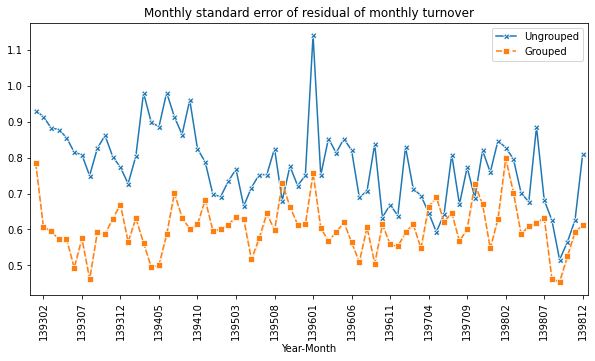
\includegraphics[width=0.85\linewidth]{Output/GroupedResSTD.eps}

	\caption{Time series of standard errors in abnormal turnover for groups}
	\label{fig:GroupedResSTD}
\end{figure}






\FloatBarrier

%
%
\subsection{{Institutional Imbalance}}

Although we provide evidence for simultaneous trade in the last section, we should show that stocks in groups that trade together are traded in the same direction. So, for each firm, we calculate daily institutional imbalances, which is the net buying value of institutional investors relative to total traded value on that day ($ \text{InsImb} = \frac{\text{Buy}_{\text{value}} - \text{Sell}_{\text{value}}}{\text{Buy}_{\text{value}} + \text{Sell}_{\text{value}}} $ [\cite{seasholes2007predictable}]). We expect that institutional imbalances have a lower variation in groups due to the correlated tradings that the ultimate owner ordered to do. So, we calculate monthly institutional imbalances for firms at the first step. As we expected, firms in the business groups have a lower level of standard error in imbalances (Panel \subref{tab:ImbalanceInsStdSummary} table\ref{st4}). Then, we calculate the monthly standard deviation of the group's imbalances and compare them to unaffiliated ones. The standard error is  $12.2\%$ and significantly (with a t-stats of 4.2) lower than ungrouped firms. 
		
	{\begin{table}[htbp]
	\caption{Summary statistics}
	\label{st4}
		\centering
		\subcaption{Panel A: Frims' Monthly Imbalances}
			\label{tab:ImbalanceInsMeanSummary}%
		\resizebox{\textwidth}{!}{
			\begin{tabular}{lrrrrrrrr}
\toprule
{} &  Group $\times$ Month &   mean &    std &  min &    25\% &    50\% &    75\% &  max \\
Grouped   &                       &        &        &      &        &        &        &      \\
\midrule
Ungrouped &                 20197 &  0.010 &  0.630 & -1.0 & -0.474 &  0.016 &  0.479 &  1.0 \\
Grouped   &                 12021 & -0.041 &  0.581 & -1.0 & -0.462 & -0.009 &  0.341 &  1.0 \\
\bottomrule
\end{tabular}

		}
	
\bigskip
		\subcaption{Panel B: Groups' Monthly Imbalances' standard erros}
				\label{tab:ImbalanceInsStdSummary}%
		\resizebox{\textwidth}{!}{
			\begin{tabular}{lcccccccc}
\toprule
{} &  Group $\times$ Month &   mean &    std &   min &    25\% &    50\% &    75\% &    max \\
Grouped   &                       &        &        &       &        &        &        &        \\
\midrule
Ungrouped &                    72 &  0.624 &  0.054 &  0.48 &  0.601 &  0.631 &  0.655 &  0.735 \\
Grouped   &                  2057 &  0.503 &  0.251 &  0.00 &  0.337 &  0.503 &  0.647 &  1.414 \\
\bottomrule
\end{tabular}

		}
\end{table}}
	\begin{figure}[htbp]
		\centering
		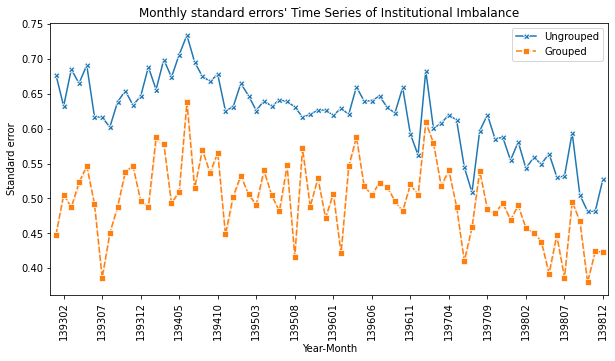
\includegraphics[width=0.85\linewidth]{Output/GroupedInsSTD.eps}
				\caption{Time series of standard errors in imbalance for groups}
		\label{fig:GroupedInsSTD}
	\end{figure}
	
	According to the main hypothesis, we need to compare pairs in groups with low standard error and other pairs. For this purpose, we define a dummy for groups whose average standard errors are lower than half of the sample;\textbf{LowImbalancestd}. So, this dummy is equal to one if at least one pair's firms belong to the low imbalance std business group. We expect pairs in the same business groups with a low standard imbalance error to move more than others. Panel \subref{Imbalance} table \ref{re4} reports estimation results and confirms that pairs in that group comove greater than others. 
	
%		{\begin{table}[htbp]
%			\centering
%			\caption{Estimation results for the relation between low imbalance std groups and comovement}
%			\label{Imbalance}
%			\subcaption{\hl{heading}}
%			\resizebox{\textwidth}{!}{
%				{
\def\sym#1{\ifmmode^{#1}\else\(^{#1}\)\fi}
\begin{tabular}{l*{6}{c}}
\hline\hline
                    &\multicolumn{6}{c}{Dependent Variable:  Future Pairs's Comovement}                                                                 \\\cmidrule(lr){2-7}
                    &\multicolumn{1}{c}{(1)}         &\multicolumn{1}{c}{(2)}         &\multicolumn{1}{c}{(3)}         &\multicolumn{1}{c}{(4)}         &\multicolumn{1}{c}{(5)}         &\multicolumn{1}{c}{(6)}         \\
\hline
SameGroup           &      0.0208\sym{***}&      0.0206\sym{***}&                     &                     &     0.00619         &     0.00630\sym{*}  \\
                    &      (7.91)         &      (7.94)         &                     &                     &      (1.95)         &      (2.04)         \\
[1em]
LowImbalanceStd     &                     &    -0.00144         &      0.0282\sym{***}&    -0.00724\sym{***}&    -0.00610\sym{***}&    -0.00267         \\
                    &                     &     (-1.15)         &      (6.06)         &     (-5.74)         &     (-4.87)         &     (-1.85)         \\
[1em]
 $ \text{LowImbalanceStd} \times {\text{SameGroup} } $ &                     &                     &                     &                     &      0.0358\sym{***}&      0.0325\sym{***}\\
                    &                     &                     &                     &                     &      (8.57)         &      (7.48)         \\
\hline
Sub-sample          &       Total         &       Total         &   SameGroup         &      Others         &       Total         &       Total         \\
Business Group FE   &          No         &          No         &          No         &          No         &          No         &         Yes         \\
Observations        &      354209         &      354209         &       43274         &      310935         &      354209         &      354209         \\
\hline\hline
\multicolumn{7}{l}{\footnotesize \textit{t} statistics in parentheses}\\
\multicolumn{7}{l}{\footnotesize \sym{*} \(p<0.05\), \sym{**} \(p<0.01\), \sym{***} \(p<0.001\)}\\
\end{tabular}
}

%			}
%	\end{table}}



		\begin{table}[htbp]
			\centering
	\caption{Turnover and Imbalance and Comovement\\ \small
				This table reports \cite{FamaMacBeth} estimates of monthly cross-sectional regressions forecasting the comovement for the sample of stocks defined in Table \ref{st1}. Other methods and definitions of variables are as in the table \ref{re1}. We also define two dummy variables for the firm's presence in the particular group. LowTurnoverStd is a dummy variable for groups in which the standard error of $\Delta \text{Turnover}$ ($ \Delta \text{Turnover}_{i,t} = \ln(\frac{\text{Turnover}_{i,t}}{\text{Turnover}_{i,t-1}}) $) is lower than the median of each period and LowImbalanceStd for a group with low dispersion in institutional imbalances ($ \text{InsImb} = \frac{\text{Buy}_{\text{value}} - \text{Sell}_{\text{value}}}{\text{Buy}_{\text{value}} + \text{Sell}_{\text{value}}} $). Controls not shown here are reported in the Internet Appendix. We report estimates of regressions using variables to investigate the effect of Turnover and Imbalance in Panel \subref{Turnovercrosssection} and Panel \subref{Imbalance}.}
				\label{re4}
				\subcaption{Low Abnormal Turnover std groups and Comovement}
				\label{Turnovercrosssection}	
			\resizebox{\textwidth}{!}{
				\centering
				{
\def\sym#1{\ifmmode^{#1}\else\(^{#1}\)\fi}
\begin{tabular}{l*{6}{c}}
\hline\hline
                &\multicolumn{6}{c}{Dependent Variable:  Future Pairs's co-movement}                                              \\\cmidrule(lr){2-7}
                &\multicolumn{1}{c}{(1)}         &\multicolumn{1}{c}{(2)}         &\multicolumn{1}{c}{(3)}         &\multicolumn{1}{c}{(4)}         &\multicolumn{1}{c}{(5)}         &\multicolumn{1}{c}{(6)}         \\
\hline
SameGroup       &   0.0208\sym{***}&   0.0210\sym{***}&                  &                  &   0.0137\sym{***}&   0.0113\sym{**} \\
                &   (7.91)         &   (7.77)         &                  &                  &   (3.73)         &   (3.19)         \\
[1em]
LowTurnoverStd  &                  & 0.000929         &   0.0171\sym{***}&-0.000982         & -0.00107         &  0.00279         \\
                &                  &   (0.84)         &   (3.88)         &  (-0.93)         &  (-1.04)         &   (1.39)         \\
[1em]
$ {\text{LowTurnoverStd} } \times {\text{SameGroup} }  $ &                  &                  &                  &                  &   0.0181\sym{***}&   0.0183\sym{***}\\
                &                  &                  &                  &                  &   (3.65)         &   (3.91)         \\
\hline
Sub-sample      &    Total         &    Total         &SameGroup         &   Others         &    Total         &    Total         \\
Business Group FE&       No         &       No         &       No         &       No         &       No         &      Yes         \\
Observations    &   354209         &   354209         &    43274         &   310935         &   354209         &   354209         \\
\hline\hline  \end{tabular}}

			}	
			\bigskip		
			\subcaption{Low Imbalance std groups and Comovement}
			\label{Imbalance}
			\resizebox{\textwidth}{!}{
				{
\def\sym#1{\ifmmode^{#1}\else\(^{#1}\)\fi}
\begin{tabular}{l*{6}{c}}
\hline\hline
                    &\multicolumn{6}{c}{Dependent Variable:  Future Pairs's Comovement}                                                                 \\\cmidrule(lr){2-7}
                    &\multicolumn{1}{c}{(1)}         &\multicolumn{1}{c}{(2)}         &\multicolumn{1}{c}{(3)}         &\multicolumn{1}{c}{(4)}         &\multicolumn{1}{c}{(5)}         &\multicolumn{1}{c}{(6)}         \\
\hline
SameGroup           &      0.0208\sym{***}&      0.0206\sym{***}&                     &                     &     0.00619         &     0.00630\sym{*}  \\
                    &      (7.91)         &      (7.94)         &                     &                     &      (1.95)         &      (2.04)         \\
[1em]
LowImbalanceStd     &                     &    -0.00144         &      0.0282\sym{***}&    -0.00724\sym{***}&    -0.00610\sym{***}&    -0.00267         \\
                    &                     &     (-1.15)         &      (6.06)         &     (-5.74)         &     (-4.87)         &     (-1.85)         \\
[1em]
 $ \text{LowImbalanceStd} \times {\text{SameGroup} } $ &                     &                     &                     &                     &      0.0358\sym{***}&      0.0325\sym{***}\\
                    &                     &                     &                     &                     &      (8.57)         &      (7.48)         \\
\hline
Sub-sample          &       Total         &       Total         &   SameGroup         &      Others         &       Total         &       Total         \\
Business Group FE   &          No         &          No         &          No         &          No         &          No         &         Yes         \\
Observations        &      354209         &      354209         &       43274         &      310935         &      354209         &      354209         \\
\hline\hline
\multicolumn{7}{l}{\footnotesize \textit{t} statistics in parentheses}\\
\multicolumn{7}{l}{\footnotesize \sym{*} \(p<0.05\), \sym{**} \(p<0.01\), \sym{***} \(p<0.001\)}\\
\end{tabular}
}

			}
			
			
		\end{table}}
\FloatBarrier

